\documentclass{beamer}

\usepackage[utf8]{inputenc}
\usepackage[T1]{fontenc}
\usepackage[english]{babel}
\usepackage{tikz}
\usepackage{algorithm}
\usepackage{algorithmicx}
\usepackage{algpseudocode}

\usetheme{default}

\newcommand{\bigO}[1]{\mathcal O \left( #1\right)}


\title{MPRI 2.19 - Programming project}
\subtitle{Analysis of cyclic attractors for \\ asynchronous boolean models of cellular networks}
\author{Marc Heinrich \and Baptiste Lefebvre}
\institute{École Normale Supérieure, Computer Science Department}
\date{February 24, 2015}


% README
% 
% Soutenance mardi 24 février entre 09h30 et 11h30.
% 
% Objectif:
%   - présenter le projet de programmation
%   - présenter qui a fait quoi pour la réalisation du projet
%   - présenter les résultats obtenus
%
% Durée:
%   - 25 minutes de présentation
%   - 15 minutes de questions


\begin{document}


\section*{Title}

\begin{frame}
  \titlepage
\end{frame}


\section*{Table of contents}

\begin{frame}
  \frametitle{Table of contents}
  \tableofcontents
\end{frame} 


% Presentation %%%%%%%%%%%%%%%%%%%%%%%%%%%%%%%%%%%%%%%%%%%%%%%%%%%%%%%%%%%%%%%%%

\section{Presentation}

\begin{frame}
  \frametitle{Presentation}    
  %Implementation of algorthms integrated in GINsim
  TODO: complete
  
  TEST: cite \cite{Bonzanni}
\end{frame}

\begin{frame}
  \begin{figure}
    % TODO: include hematopoietic in folder img
    %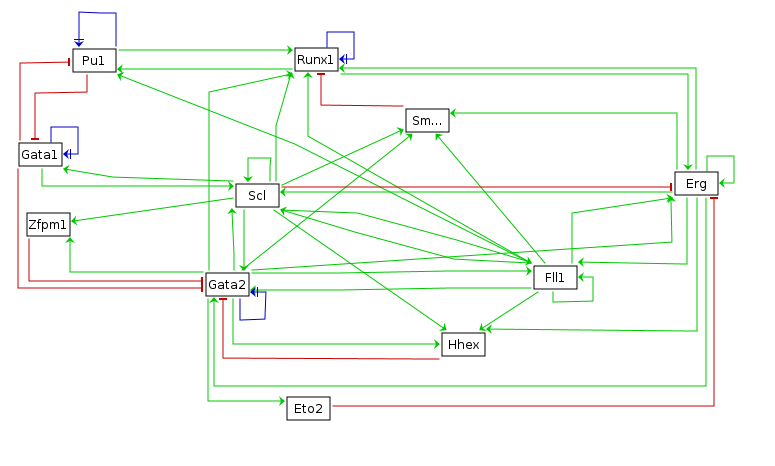
\includegraphics[scale=0.4]{hematopoietic}
    \caption{Boolean Model for blood stem cells}
  \end{figure}
\end{frame}

\subsection{Introduction to MDDs}
% Maybe not put here
% Slides from previous presentation
\begin{frame}
  % 2 minutes... probably 3 actually
  \frametitle{BDDs/MDDs}
  Représentation compacte d'une fonction booléenne à $n$ variables.
  
  \begin{figure}
    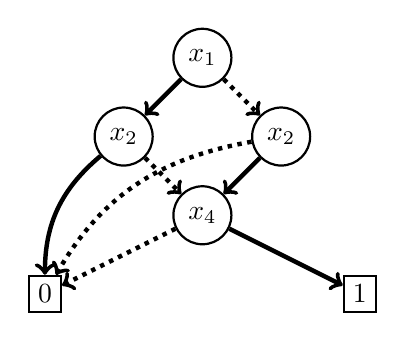
\begin{tikzpicture}
      \tikzstyle{endnode} = [draw, rectangle, thick, black] ;
      \tikzstyle{varnode} = [draw, circle, thick, black] ;
      \tikzstyle{onearrow} = [->, ultra thick, black] ;
      \tikzstyle{zeroarrow} = [->, ultra thick, black, dotted] ;
      \node[varnode] (x1) at (0,0) {$x_1$} ;
      \node[varnode] (1x2) at (-1,-1) {$x_2$} ;
      \node[varnode] (2x2) at (1,-1) {$x_2$} ;
      \node[varnode] (x4) at (0,-2) {$x_4$} ;
      \node[endnode] (1) at (2,-3) {1} ; 
      \node[endnode] (0) at (-2,-3) {0} ;
      \draw[onearrow] (x1) -- (1x2) ;
      \draw[onearrow] (1x2) to[out=-140, in=90] (0) ;
      \draw[onearrow] (x4) -- (1) ;
      \draw[onearrow] (2x2) -- (x4) ;
      \draw[zeroarrow] (x1) -- (2x2) ;
      \draw[zeroarrow] (2x2) to[out=-170, in = 60] (0) ;
      \draw[zeroarrow] (1x2) -- (x4) ;
      \draw[zeroarrow] (x4) -- (0) ;
    \end{tikzpicture}
  \end{figure}

  \begin{definition}
    MDD : Extension to multivalued variables
  \end{definition}
\end{frame}

\begin{frame}
  \frametitle{Operations on MDDs}
  \begin{itemize}
  \item Apply binary operators (ex: AND, OR, EQUAL, ....)
    \bigskip
  
  \item Apply existential/universal quantifiers
    \bigskip
  
  \item Substitute variables
    \bigskip
  
  \item Composition of functions
    \bigskip
  
  \item Comparison of MDDs
    \bigskip
  
  \item Find satisfying assignments
  \end{itemize}
\end{frame}

\begin{frame}
%Mettre l'intérêt de cette structure de données
  \begin{block}{Pros}
    \begin{itemize}
    \item Compact representation of Boolean/Integer functions
    \item Represent a set of states by its indicator function.
    \end{itemize}
  \end{block}
  
  \bigskip
  \begin{block}{Cons}
    \begin{itemize}
    \item De taille potentiellement exponentielle
    \item La taille dépend de l'ordre des variables
    \end{itemize}
  \end{block}
\end{frame}


% Distribution of tasks %%%%%%%%%%%%%%%%%%%%%%%%%%%%%%%%%%%%%%%%%%%%%%%%%%%%%%%%

\section{Distribution of tasks}

\begin{frame}
% 1 minute
  \frametitle{Distribution of tasks} 
  Implementation of different modules for GINsim
  
  \begin{itemize}
  \item Finding minimum perturbation
    \bigskip
    
  \item MDD based algorithm for computing attractors
    \bigskip
    
  % TODO : better description
  \item LIP based algorithm for computing attractors
  \end{itemize}
\end{frame}

\begin{frame}
  % 2- minutes
  % explain problem
  \frametitle{Finding the minimum perturbation}
  \begin{block}{Problem}
    Given a set of initial states, find the minimum perturbation that allows to reach a given target state.
    
    Reformulation : among the ancestors of the target state, find the closest to the source.
  \end{block}
\end{frame}

\begin{frame}
  % TODO: explain example Bonzanni
  \begin{figure}
    % TODO: include push in folder img
    %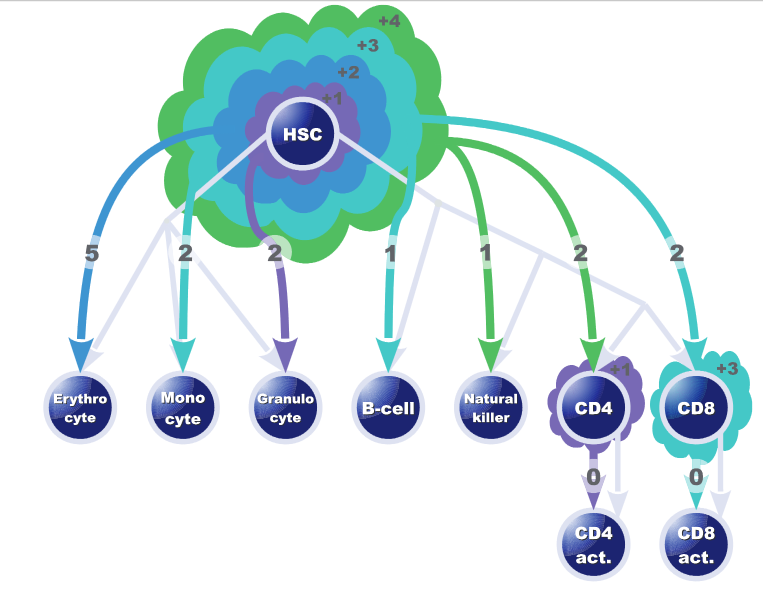
\includegraphics[scale=0.35]{push}
    \caption{Minimum perturbations for the model from Bonzanni et al.}
  \end{figure}
\end{frame}

\begin{frame}
  \frametitle{Solution}
  \begin{itemize}
  \item Compute the set of ancestors of the target state.
    \bigskip
    
  \item ennumerate all these states to find the closest
  \end{itemize}
  \bigskip
  
  \onslide<2>
  \begin{block}{Improvement}
    Use only MDDs to compute the minimum number of genes to modify.
  \end{block}
\end{frame}


\begin{frame}
% 3-4 minutes
  \frametitle{Finding attractors}
  \begin{definition}
    An attractor is a set of states that has no outbound transition, minimal for inclusion.
  \end{definition}
\end{frame}

\begin{frame}
  \frametitle{MDD formulation}
  \begin{block}{}
    Given a model, we represent it using MDDs by its transition function $f$:
    $$ f(x,y) =1 \Leftrightarrow x \rightarrow y$$
  \end{block}
  
  \begin{block}{Successor}
    The successors of a set of state $s(x)$ are the states $y$ that satisfy the MDD:
    $$ \exists x, s(x) \wedge f(x,y)$$
  \end{block}
  
  \begin{block}{Predecessor}
    The predecessors of a set of state $s(y)$ are the states $x$ that satisfy the MDD:
    $$ \exists y, s(y) \wedge f(x,y)$$
  \end{block}
\end{frame}

\begin{frame}
  %Synchronous algorithm
  \frametitle{Synchronous algorithm}
  
  \begin{block}{Notations}
    \begin{itemize}
    \item $FR(x) = \{ y,  x \rightarrow^* y \}$ : descendants 
    \item $BR(x) = \{ y, y \rightarrow^* x \} $ : ancestors
    \end{itemize}
  \end{block}
  
  \bigskip
  \begin{algorithmic}
    \State $states \gets \mathcal S$
    \State $Att_{syn} \gets \emptyset$
    \While{$states \neq \emptyset$}
      \State $x \gets \text{FindState}(states)$
      \State $Att_{syn}.add(FR(x))$
      \State $states \gets states \setminus BR(x)$
    \EndWhile
  \end{algorithmic}
  
\end{frame}

\begin{frame}
  %Asynchronous algorithm
\end{frame}

\begin{frame}
  % Bapt : LIP based algo
  TODO
\end{frame}


% Results %%%%%%%%%%%%%%%%%%%%%%%%%%%%%%%%%%%%%%%%%%%%%%%%%%%%%%%%%%%%%%%%%%%%%%

\section{Results}

\begin{frame}
  \frametitle{Results}
  %Demonstration on GINsim of the different plugins?   
  TODO: complete
\end{frame}


\section*{References}

\begin{frame}
  \frametitle{References}
  \bibliographystyle{apalike}
  \bibliography{presentation.bib}
\end{frame}


\end{document}
